\chapter{Background}
\label{cha:relatedwork}
\chapterquote{Authentication is the process of determining whether someone or something is, in fact, who or what it is declared to be}{D.R. Patel - INFORMATION SECURITY: Theory and Practice}

In this section, the global system known as \emph{devices cloud} will be first detailed. Afterwards, the reader will be introduced to the different possible protocols and technologies that could be used and an overview of the different researches and studies that have been previously performed will be given.
 
\section{The Devices Cloud}
Integrating the requirements defined in the Introduction to a more detailed view of the global system, the architecture the Figure \ref{fig:design_complete} of the \emph{devices cloud} architecture can be rendered. Of course, only the information relevant for this thesis is depicted.

\begin{figure}[!ht]
	\centering
	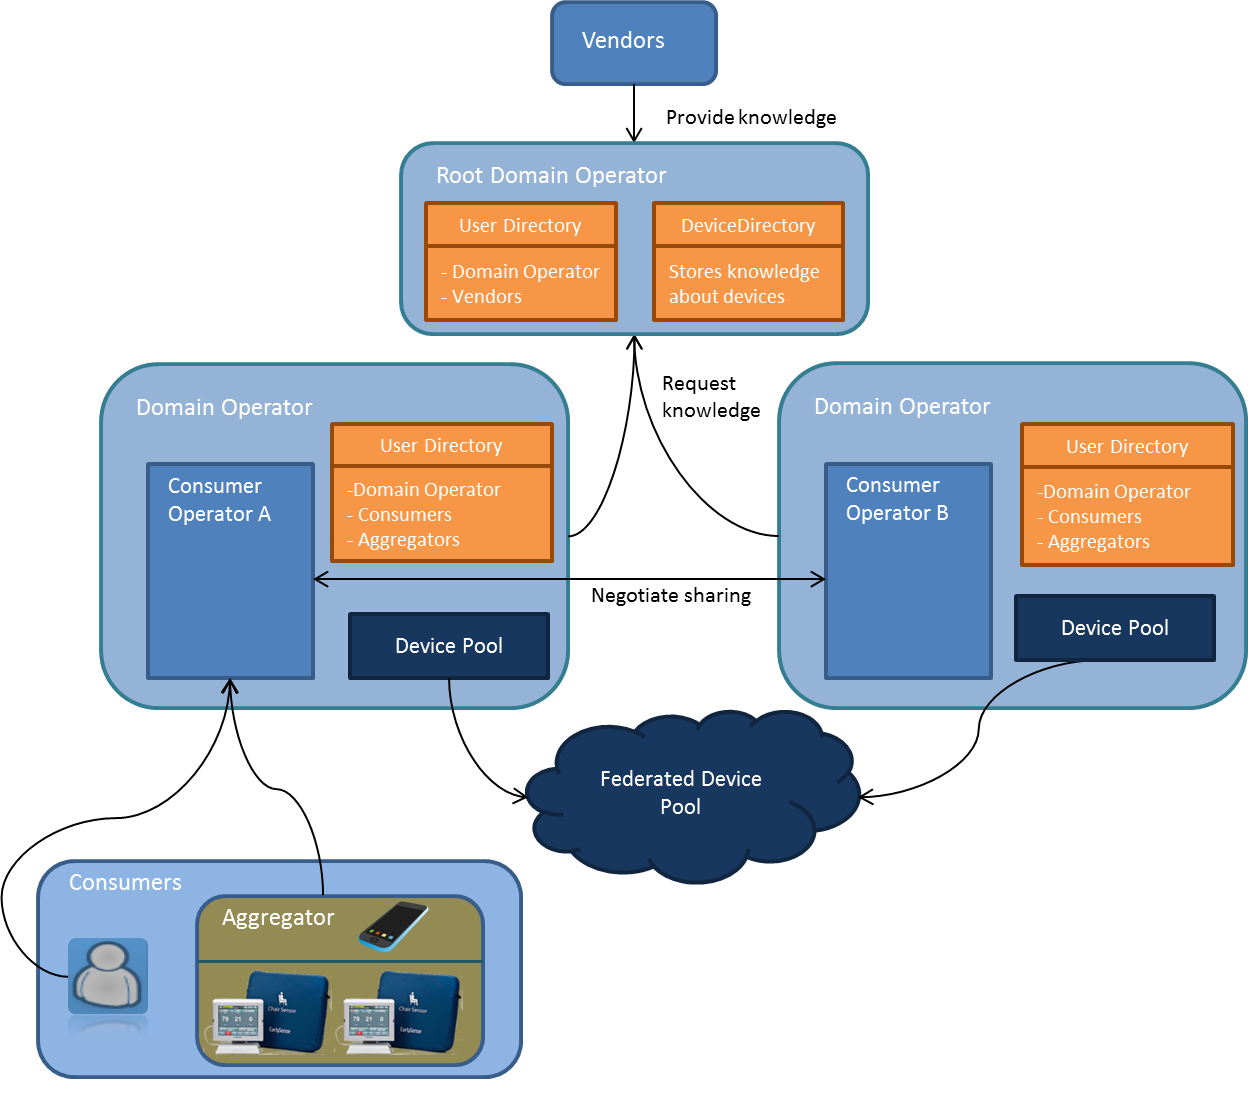
\includegraphics[scale=0.3]{images/design_complete}
	\caption{Detailed Architecture of the Devices Cloud}
	\label{fig:design_complete}
\end{figure}

Every Domain Operator maintain a User Directory and a Device Directory. The earlier is used to authenticate and authorize every entities that can be. The latter is used to store the information about every device operated by the operator.

The Device Directory is particularly important for authorization purposes, because it stores knowledge like the Device Owner and Device Operator for every device. As explained in the Introduction, those two roles are the only ones that are authorized, for example, to revoke a device's access. 

In the framework, the Device Directory could then be compared to the authorization server in the sense that it can map an entity with roles.

This Device Directory has a public interface, the Device Pool, containing the devices they operate. This Device Pool contains only the information that an end customer can see in order to choose which devices he wants to have access to. The different device pools contribute then to a Federated Device Pool, containing all devices available to the customers. Those, when registered to their Domain Operator, can have access to this Federated Pool. Of course, the different pools of devices must be synchronized, but it will not be explained in this thesis.

When a customer has chosen which devices he wants to read the data from, he uses an aggregator, most likely its mobile phone, to integrate the different devices. The authentication of the different actors is first performed (intra Operators, between Customer and Domain Operator, ...), the required data (like drivers) is then retrieved from the Domain Operators or Root Domain Operator and the data can eventually be read from the device.

 \subsection{Entities}
 In \citetitle{reference_thesis}, four main characteristics have been defined for the entities present in the \emph{device cloud}:
 
% \begin{table}[!ht]
% 	\caption{Type of Entities in the Device Cloud}
%	 \centering
	 \def\arraystretch{1.5}
%	 \setlength{\extrarowheight}{15pt}
	 \begin{longtable}{|m{\textwidth}|}
	 	\caption{Type of Entities in the Device Cloud} \\
	 	\hline
	 	\rowcolor{Gray}\textcolor{white}{\textbf{  Entities Characteristics}}
	 	\\ \hline

		
	 	\pbox{\linewidth}{
	 		\vspace*{10pt}
		 	 \textbf{Attachment Entity:} \\
	 		 An attachment refers to any kind of resource usually stored on the file system (e.g.	a picture or a binary). Attachment Entities can have several attachments.
	 		}
	 		\\ \hline
	 	
	 	\pbox{\linewidth}{
	 		\vspace*{10pt}
	 		\textbf{Configurable Entity:} \\
	 		A configurable entity holds a set of configuration entries expressed as key-value pairs. Each entry again is backed by the global entity definition (in the Root Domain). This means, that each local copy of an entity can have two virtual sets of configuration entries.
	 	} \\
 	\hline
 		\pbox{\linewidth}{
 			\vspace*{10pt}
 			\textbf{Location Tagged Entity:} \\
 			An entity whose location can be monitored. This can be an important parameter
 			when having to decide about competing device access re quests or requests to devices
 			that are already provisioned. 
 		} \\
 		\hline
 		\pbox{\linewidth}{
 			\vspace*{10pt}
 			\textbf{Principal Entity:} \\
 			A Principal Entity is an entity that can be authenticated by the User Directory using its EntityID and some kind of security credentials (e.g. certificate or password).
 			Examples are Consumer Operators, Consumers, Aggregators or Vendor. 
 		} \\
 		\hline
 \end{longtable}
 
 in this thesis, the focus will be put on Principal Entities, since it's the most relevant characteristic when designing an authentication framework. However, an entities can have several characteristics at the same time. Every type of entity must then be taken into consideration.
 
 Based on the \emph{device cloud}, a non-exhaustive list of the entities that must maintained the User Directory has been determined:
 
  \def\arraystretch{1.5}
  %	 \setlength{\extrarowheight}{15pt}
  \begin{longtable}{|m{\textwidth}|}
  	\caption{User Directory Entities} \\
  	\hline
  	\rowcolor{Gray}\textcolor{white}{\textbf{  User Directory Entities}}
  	\\ \hline
  	
  	\pbox{\linewidth}{
  		\vspace*{10pt}
  		\textbf{Aggregator:} \\
  		Used for authenticating Aggregators within a Domain.
  	}
  	 \\
  	 Inherit from: Attachment Entity, Configurable Entity, Principal Entity, Location Tagged Entity.
  	\\ \hline
  	\pbox{\linewidth}{
  		\vspace*{10pt}
  		\textbf{Consumer:} \\
		Used for authenticating Consumers within a Domain. 
  	} 
  	\\
  	Inherits from: Attachment Entity, Configurable Entity, Principal Entity, Location Tagged Entity.
  	\\	\hline
  	\pbox{\linewidth}{
  		\vspace*{10pt}
  		\textbf{Consumer Profile:} \\
  		The Consumer Profile is bound to a Consumer and stores preferences or predefined configurations.  
  	} 
  	\\
  	Inherits from: Attachment Entity, Configurable Entity.
  	\\ 	\hline
  	\pbox{\linewidth}{
  		\vspace*{10pt}
  		\textbf{Operators:} \\
  		Used for authenticating Operators within a Domain and store required information, like how to communicate with the Operator. In order to do so, the two following properties have been defined:
  	}
  	\\
  	
  	 \hspace{2em}\hangindent=2em \tabitem \textit{DomainOperator}: flag indicating whether the Operator is a Consumer or a Domain Operator.
  	\\
  	\hspace{2em}\hangindent=2em	\tabitem \textit{ProtocolURI}: defines the endpoint where to contact the Operator (protocol + location), most of the time an absolute URL. 
  	\\
  	Inherits from: Attachment Entity, Configurable Entity, Principal Entity. 
%  	\pbox{\linewidth}{
%  		\vspace*{10pt}
%  		\textbf{Operators:} \\
%  		Used for authenticating Operators within a Domain and store required information, like how to communicate with the Operator. In order to do so, the two following properties have been defined:\\
%  		% 		\begin{itemize}
%  		%  			\item \textit{DomainOperator}: flag indicating whether the Operator is a Consumer or a Domain Operator.
%  		%  			\item \textit{ProtocolURI}: defines the endpoint where to contact the Operator (protocol + location), most of the time an absolute URL. 
%  		%  		\end{itemize}
%  		
%  		Inherits from: Attachment Entity, Configurable Entity, Principal Entity.
%  	} 
  	\\	\hline
  	\pbox{\linewidth}{
  		\vspace*{10pt}
  		\textbf{Vendors:} \\
  		Used for authenticating Vendors within a Domain.
  	} 
  	\\
  	Inherits from: Attachment Entity, Configurable Entity, Principal Entity.
  	\\	\hline
  \end{longtable}
 
In addition to the four entities that must be authenticated, a consumer Profile has been added. this profile is used for storing predefined set of devices that a user needs and the different modules needed for processing the data. To make it clear, let's take the example of a diabetic A who had a brand new sensor installed for measuring the blood glucose level(Google contact lenses, or Apple iWatch for example).

The hospital B is quite familiar with those technologies, but it wishes that the data retrieved can be immediately readable with the CSV format, and not with the proprietary format of Google or Apple. In that case, the hospital can set up a profile where the device (the new sensor) is defined, as well as the module that converts the proprietary format into CSV format.
\linebreak
\linebreak
\linebreak
The reader should now have a good knowledge of the global design and its requirements. The next section introduces him to the authentication and authorization principles and implementations.

\section{Encryption}
Encryption is one of the key principle of network security. It ensures that nobody can have access to protected information even if a message has been intercepted, by encoding the messages. Different algorithms and methods exist, so that only the recipient of a message can decrypt the encoded message.

\subsection{symmetric key}
\label{sec:02_symmetric_keys}
Some algorithm or protocols are based on a symmetric key. It is assumed that both the sender and the recipient of the messages share a secret (the key). Only the two actors A and B can then encrypt and decrypt the messages thanks to this shared secret key.

Of course, it is assumed that the underlying cryptosystem is strong, so that nobody can decrypt the messages without the key.

This system requires also that the two communicating entities share the secret key from the beginning, which poses the problem of the key distribution. This can be done through physical delivery (A delivers the key to B, or a third party delivers a key to A and B), by using a previous shared key (the new key is sent encrypted with the old key), or by using an encrypted communication with a third party C.
 
\subsection{asymmetric keys}
Other algorithms are based on asymmetric keys. This time, every entity has two keys: a public one $k_{p}$, that can be sent to anybody, and a private $ k_{p}^{-1} $, that is kept secret.

The idea underneath this system is that a message encrypted with $k_{p}$ can only be decrypted with $ k_{p}^{-1} $, and, the other way around, a message encrypted with $ k_{p}^{-1} $ can only be decrypted with $k_{p}$.

Since the public key is accessible to anybody, an asymmetric key based system doesn't show the same key distribution problem.

\subsection{SSL}
SSL is described\cite{freier2011secure} as a protocol that "allows client/server applications to communicate in a way that is designed to prevent eavesdropping, tampering, or message forgery".

The symmetric key encryption is simpler and quicker than the asymmetric one, but asymmetric encryption is more resilient to attacks. SSL uses therefore asymmetric keys to build a symmetric key. This functioning is explained in the following simplified sequence:

\begin{enumerate}
	\item The client connects to the server and asks for authentication.
	\item The server sends a certificate, signed by a certificate authority (CA) and containing the public key of the server.
	\item The client checks with the CA if the certificate is valid. If it is, the server is assumed to be a trusted server providing secure service (like online billing).
	\item The client generates a random session key, signs it with the server's public key and send it to the sever.
	\item The server can decrypt the session key with its private key.
\end{enumerate}

It is here presupposed that a certificate authority exists. This can be a dedicated one (in this case, a standard browser would notify that the certificate is not secure) or a recognized one. In the latter case, every server has to buy a certificate from a known authority. The creation, verification and revocation of certificates requires a Public Key Infrastructure (PKI) to be established.

SSL is also a protocol that lies between the transport layer (like TCP) and the application layer of the OSI model. It means, the process is completely transparent to the user and is done automatically. The most basic example is the online billing. When a user pays in Amazon, for example, he doesn't notice that it is using SSL, it is done automatically by the browser.

it is therefore not unusual that an authorization and authentication process is implemented on top of a SSL secured connection.


\section{Authentication}
Authentication, as aforementioned, can rely on encryption, but other approaches are possible. This section aims at explaining what is authentication, and giving an overview of the different possible protocols. 

\subsection{Principles}
As explained in \citetitle{patel2008information}\cite{patel2008information}, authentication is the process of determining whether someone or something is, in fact, who or what it is declared to be.	In order to do so, the server needs to check the authenticity of a piece of information. This can be done through the following verification types:

\begin{description}
	\item[Proof by Knowledge] The user must send information that only he is supposed to know. It can be a password / login, or a challenge from the server for example (the user must answer to some questions, or recognize patterns, etc).
	\item[Proof by Possession] The user authenticate with a property that only he is supposed to have. Examples are electronic ID cards or one time passwords on the mobile phone.
	\item[Proof by Property] Something that the user is or does. It could be for instance DNA, retina, fingerprint, or signatures. 
\end{description}

For a more secure authentication, the above listed factors can be combined. The banking terminals, for example, are based on a knowledge and an ownership factor. The user must possess its card and know a PIN code.

In regards to this thesis, only knowledge factors can be observed. On one hand, the Customers, Vendors have credentials, and can thus authenticate with a login / password. Aggregators and Operators, in the other hand, are not human being and cannot enter credentials. Details about their authentication will be given in section \ref{cha:03:design_concept}.

%Furthermore, two authentication types exist: the mutual authentication, where two parties authenticate within each other during the same process, and one-way authentication. Given the architecture and requirements of the \emph{device cloud}, only one-way authentication will be detailed. 

\subsection{Based on a symmetric key}
In a symmetric cryptosystem, a principal can indifferently encrypt and decrypt with its key. Without the knowledge of this key, an entity cannot create an encrypted message or decrypt an already encrypted one. Hence, the following authentication principle, called \emph{SYM}, can be deducted\cite{Woo1997}:

\begin{quote}
	\textit{If a principal can correctly encrypt a message using a key that the verifier believes is known
	only to a principal with the claimed identity (outside of the verifier), this act constitutes sufficient proof of identity}
\end{quote}

The most basic authentication, with P and Q the two parties, can be thus proceeded as follows:

\begin{tabbing}
	\hspace{4em}\=\hspace{4em}\=\hspace{2em}\=\kill
	\>  P \>  : \> create $m =$ "I am P" \\
	\>    \>  : \> compute $m' = \lbrace m, Q \rbrace_{k}$ 				\\
	\>  P $\rightarrow$ Q \>  : \> $m,m'$ \\
	\>  Q \>  : \> verify $\lbrace m, Q \rbrace_{k} = m'$ \\
		\>    \>  : \> if equal then accept, else reject \\
\end{tabbing} 

One of the main weakness of this sequence is replay attack. Indeed, if an entity could access the message $m,m'$ of the third step, it could send it to Q later on and thus masquerade P.

The use of nonce or timestamps can then be used for protecting against those replay attacks:

\begin{tabbing}
	\hspace{4em}\=\hspace{4em}\=\hspace{2em}\=\kill
	\>  P $\rightarrow$ Q\>  : \> create $m =$ "I am P" \\
	\>  Q  \>  : \> generate nonce $n$	\\
	\>  Q $\rightarrow$ P \>  : \> $n$ \\
	\>  P  \>  : \> compute $m' = \lbrace P, Q, n \rbrace_{k}$ 				\\
	\>  P $\rightarrow$ Q \>  : \> $m$ \\
	\>  Q \>  : \> verify $\lbrace P, Q, n \rbrace_{k} = m$ \\
	\>    \>  : \> if equal then accept, else reject \\
\end{tabbing} 

If an entity now replay the message $\lbrace P, Q, n \rbrace_{k}$, the nonce will not be valid anymore and thus successful replay attacks can be avoided.

In regards to the choice between timestamps and nonce, it should be understood that the use of timestamps requires every entities clock to be synchronized, which might be difficult when the number of clocks gets high. Besides, if the replay attacks is executed fast enough, the timestamps could still be valid. Therefore, nonce are in general to be preferred.
\label{02_timestamp_vs_nonce}

When using such a symmetric cryptosystem, it is supposed that there exists one key per pair of entities. In a network of N entities, this would rise up to $\frac{N.(N-1)}{2}$ keys. In addition, every entity would have to maintain N keys. The scalability of the process is therefore not optimal. 

For this reason, in the majority of the proposed protocols for distributed systems, a centralized authentication server A is introduced. This server shares a key $K_{X,A}$ with every other entity X. A lot of protocols have been proposed, many based on the one put forth by Needham and Schroeder\cite{needham1978using}. It has been improved for example twice by Denning\cite{denning1981timestamps}\cite{robling1982cryptography}, adding timestamps. 

One could consider in the end a protocol as follows (with P, Q the two parties and A the centralized authentication server):

\begin{tabbing}
	\hspace{4em}\=\hspace{4em}\=\hspace{2em}\=\kill
	\>  P $\rightarrow$ Q \>  : \> "I am P" \\
	\>  Q  \>  : \> generate nonce $n$ \\
	\>  Q $\rightarrow$ P \>  : \> $n$ \\
	\>  P  \>  : \> compute $x = \lbrace P, Q, n \rbrace_{k_{P,A}}$ 				\\
	\>  P $\rightarrow$ Q \>  : \> $x$ \\
	\>  Q  \>  : \> compute $y = \lbrace P, Q, x \rbrace_{k_{Q,A}}$ 				\\
	\>  Q $\rightarrow$ A \>  : \> $y$ \\
	\>  A  \>  : \> recover $P,Q,x$ from $y$ with $k_{Q,A}$ \\
	\>    \>  : \> recover $P,Q,n$ from $x$ with $k_{P,A}$ \\
	\>    \>  : \> compute $m = \lbrace P,Q,n \rbrace_{k_{Q,A}}$ \\
	\>  A $\rightarrow$ Q \>  : \> $m$ \\
	\>  Q \>  : \> verify $\lbrace P, Q, n \rbrace_{k_{Q,A}} = m$ \\
	\>    \>  : \> if equal then accept, else reject \\
\end{tabbing} 

Q uses A for translating a message encrypted with P's key to a message only encrypted with Q's key. This way, only N keys must be maintained. The major securities issues are here reported to the authorization server A, which must be protected with strong security systems.

It must also be noted that the protocols described here are used only to check if the sender of a message is authentic. The following connections can then be facilitated with the creation of a session key, but it will not be detailed here.

\subsection{Based on asymmetric keys}
With an asymmetric cryptosystem, an entity P is the only one able to sign messages with $k_{P}^{-1}$, since it is supposed to be kept secret. Thus, if the decryption of a message by $k_{P}$ makes sense, it means that the message originally came from P. The principle \emph{ASYM} can be deducted\cite{Woo1997}:

\begin{quote}
	\textit{If a principal can correctly sign a message using the private key of the claimed identity, this act constitutes a sufficient proof of identity.}
\end{quote}

Similarly to the symmetric cryptosystem, a basic protocol can be conceived this way:

\begin{tabbing}
	\hspace{4em}\=\hspace{4em}\=\hspace{2em}\=\kill
	\>  P $\rightarrow$ Q\>  : \> "I am P" \\
	\>  Q  \>  : \> generate nonce $n$	\\
	\>  Q $\rightarrow$ P \>  : \> $n$ \\
	\>  P  \>  : \> compute $m = \lbrace P, Q, n \rbrace_{k_{P}^{-1}}$ 				\\
	\>  P $\rightarrow$ Q \>  : \> $m$ \\
	\>  Q \>  : \> verify $(P,Q,n) = \lbrace m \rbrace_{k_{P}}$ \\
	\>    \>  : \> if equal then accept, else reject \\
\end{tabbing} 

Again, in a distributed network with N nodes, every node would have to maintain the public keys of the other entities. A centralized authentication server A can be inserted into the above described protocol:

\begin{tabbing}
	\hspace{4em}\=\hspace{4em}\=\hspace{2em}\=\kill
	\>  P $\rightarrow$ Q\>  : \> "I am P" \\
	\>  Q  \>  : \> generate nonce $n$	\\
	\>  Q $\rightarrow$ P \>  : \> $n$ \\
	\>  P  \>  : \> compute $m = \lbrace P, Q, n \rbrace_{k_{P}^{-1}}$ 				\\
	\>  P $\rightarrow$ Q \>  : \> $m$ \\
	\>  Q $\rightarrow$ A \>  : \> "I need P's public key" \\
	\>  A \>  : \> retrieve P's public key $k_{P}$ \\
	\>  A \>  : \> create certificate $c = \lbrace P, k_{P} \rbrace_{k_{A}^{-1}} $ \\
	\>  A $\rightarrow$ Q \>  : \> $P,c$ \\
	\>  Q \>  : \> verify $(P,Q,n) = \lbrace m \rbrace_{k_{P}}$ \\
	\>    \>  : \> if equal then accept, else reject \\
\end{tabbing} 

Here, c, a \emph{public key certificate} is the belief that P's public key is $k_{P}$. In such a system, the different entities don't have to know the public keys of everyone from the beginning. Hence, the key distribution problem underlined in the section \ref{sec:02_symmetric_keys} can be avoided. However, a PKI has to be set up.

\subsection{Based on a One-way function}
Another possibility to authenticate principals is to rely on a so-called One-way function, and no more on key based encryption.

\subsubsection{One-Way function}
Such a function $f$ presents the following properties:
\begin{itemize}
	\item \textbf{Easy to compute:} \\
	it can be computed in a polynomial time algorithm.
	\item \textbf{Hard to invert:} \\
	from ($f(x)$) only, finding a corresponding $x$ must be difficult. In mathematical terms,  for every randomized algorithm $A$ that runs in time polynomial in $n=|x|$, every polynomial $p(n)$, and all sufficiently large $n$: \\
	$ P_{r}[f(A(f(x))) = f(x)] < \dfrac{1}{p(x)}$ 
	\item \textbf{(Optional) collision-free:} \\
	it is unfeasible to find a collision, i.e. $f(x) = f(y)$ and $x \ne y$.
\end{itemize}

Similarly to the symmetric cryptosystem, it is assumed that the two communicating entities know the One-way function. The advantage of those functions in regards to a symmetric key is that it can be more easily designed than an encryption algorithm, since they don't have to be invertible, but only present the collision-free property. Indeed, for authentication, the collision-free property is particularly important because it is the only way to check the authenticity of a message.

\subsubsection{Proposed protocol}
One of the most famous protocols using one-way functions has been proposed by Li Gong\cite{Gong1989} in \citetitle{Gong1989}.

In this protocol, the two parties share a secret with a centralized server A. Combined with nonces and secrets, 2 different one-way functions ensure that, after a 5 steps sequence, P and Q share a fresh secret that nobody else could have discovered.

The use of such functions doesn't reduce capabilities of authentication systems, and can facilitate computation. They could also be use in a more elaborated authentication scheme, like a Kerberos-like system (see section \ref{sec:02_Kerberos}).

\subsection{Password authenticated key exchange - PAKE}
The password authenticated key exchange is an interactive method for two parties to create a session key based only on the knowledge of a password. This method doesn't require any PKI (it doesn't use SSL, for example) but ensure a secure communication.

Unlike SSL based authentication, it is also not subject to man-in-the-middle attack. Indeed, if a user discloses its password on a phishing website, even if the session is SSL encrypted, the password will be stolen. In PAKE, the password is never revealed, only proofs of its knowledge are sent through the network.

The first milestone occurred in 1992 when Bellovin and Merrit designed the EKE protocol\cite{Bellovin1992}. This protocols has been proven to have several weaknesses, but it showed at least that the idea underneath PAKE could be implemented. Many algorithm have been afterwards proposed, of which several were variants of the EKE protocol. In 2008, stating that the few methods that were said to be resilient to known attacks were patented (EKE\cite{bellovin1993cryptographic} and SPEKE\cite{jablon2001cryptographic}), F. Hao and Peter Ryan proposed J-PAKE (Juggling) which is proven to be secure\cite{hao2010j}\cite{Hao2011}. Nevertheless, It is restricted to only two communication parties, whereas other protocols allow for a trusted third party to mediate between the two communicating parties for mutual authentication\cite{gong1993protecting}\cite{gong1995optimal}.

Even authentication between realms could be performed with PAKE \cite{byun2002password}. In a distributed environment like the \emph{device cloud}, where service providers authenticate their user and cooperate for remote user authentication, this is a possibility. However, several flaws have been discovered \cite{Wang2004}.

The main drawback that a PAKE system could have is that it requires that every pair of entities share a secret (like a password) from the beginning. This hypothesis can in practice become a unpractical, as the number of network nodes gets high and if the nodes can be dynamically integrated into the network.


\subsection{Shared Authentication Framework}
This section focus on frameworks that provide a unified authentication throughout a distributed system, with the most transparent from the end-user's point of view. Those systems can for instance rely on a protocol described above, but enhance this one with a global design and infrastructure. 

In a shared authentication framework, the services collaborate together to provide a transparent authentication service. Two concepts must here be distinguished: Single-Sign-On (SSO) and Federated Identity Management (FIM).

\subsubsection{TODO: Trust ?}

\subsubsection{SSO}
\label{sec:02_SSO}
SSO (Single-Sign-On) is a feature of a set of services, with which a user enters only once its credential for being able to access all services contained in the set, even when those services are not delivered by the same organization.
\\
 
\quad \tabitem	\textbf{Kerberos}

\label{sec:02_Kerberos}
Kerberos\cite{Sundareswaran} is a computer network authentication service developed as part of the Project Athena at MIT, and still today the leading service in the enterprise universe. Two major versions exist, the v4 and v5, which is known to make up for some weaknesses in the v4 version. Kerberos is based on the use of tickets, with which entities prove their identity, and it relies on symmetric encryption.

The following entities are defined:
\begin{description}
	\item[Client]: the user to authenticate (and its client, like a web browser).
	\item[Key Distribution Server (KDS)]: the Kerberos organization that delivers the different Kerberos services. Most of the time, it encompasses an Authentication Server and a Ticket Granting Server.
	\item[Authentication Server (AS)]: the Kerberos server that authenticates the client. It delivers access tickets to the TGS.
	\item[Ticket Granting Service (TGS)]: the Kerberos server that delivers tickets for a specific service and a specific user.
	\item[Service Server (SS)]: the service the user wants to have access to. 
\end{description}

The simplified authentication flow is depicted in Figure \ref{fig:kerberos_simple}.

\begin{figure}[!ht]
	\centering
	\caption{Kerberos authentication flow}
	\label{fig:kerberos_simple}
	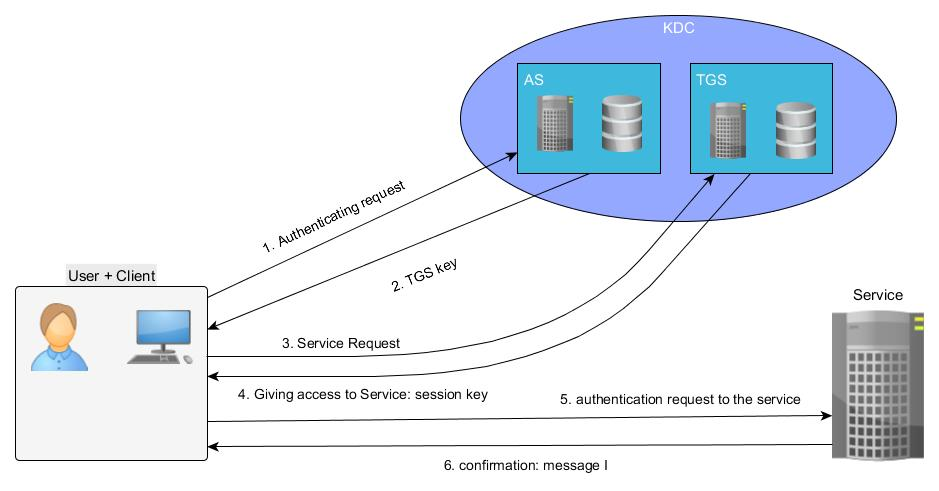
\includegraphics[scale=0.4]{images/kerberos_simple}
\end{figure}

The idea behind Kerberos is to provide registration for both the users and the services. This would be done by the Key Distribution Center in respectively the AS and the TGS.

That way, a user first authenticates with the AS, and receives a key for communicating with the TGS. It can then request the TGS for a specific service SS. If the service is known to the TGS, the TGS returns a session key for the communication between the user and SS. 

A more detailed overview of the process is given in \hyperref[appendix:kerberos]{Appendix 2}.

Kerberos is still the leader in the authentication frameworks world. However, it shows some weaknesses. M. Belovin \textit{et Al.} analyzed Kerberos v5\cite{Bellovin1990} and its inherent weaknesses. He found several potential weaknesses, like replay attacks (the protection against replays is based on timestamps, which are not very secure, as explained in section \ref{02_timestamp_vs_nonce}), spoofing login (the end workstation is corrupted and save login and credential on login), password guessing attack, or ticket scope (a KDC defines a Kerberos \textit{realm}, but several realms can be connected, and the KDC cooperate for authenticating users from remote realms. Every realm can have a trust policy about which other realms it can trust. But if a realm A trusts a realm B, which trusts a realm C, then A will trust C, even if the policy of A is against that).

Even if some corrections have been implemented (nonces have been added as an extra security feature for example), the Kerberos protocol still remains under the threat of password guessing attack, for example. In 2009, \cite{kim2009survey} M. Kim explains that Kerberos v5 uses a pre-authentication scheme in order to prevent off-line password attack. But if an attacker can access enough of those pre-authentication messages, it could execute a dictionary attack. Indeed, the message sent by the server consists in a timestamp, encrypted with a key derived from the user's password, and the timestamp always have the same format YYYYMMDDHHMMSSZ.

The paper also present another strong weakness to a man-in-the-middle attack, by setting up a fake KDC. Concerning this specific attack, B. Hill explained that even if the authentication protocol is seconded by strong authentication measures, like smart card reader authentication,  the attack can still be successfully executed to masquerade users\cite{Consultant}.
\\

\quad \tabitem \textbf{SPX}

SPX\cite{Tardo1991} is a self-contained implementation of a distributed authentication service. SPX doesn't require trust relationships between components and is on the contrary aimed at handling those relationship between mutually suspicious authorities. SPX works with the use of ISO/CCITT X.509 Directory Authentication, which involves a PKI.

SPX is composed of:
\begin{itemize}
	\item a run-time library providing the principals with access to the authentication services.
	\item The Certificate Distribution Center (CDC) which distribute public key and other authentication information.
	\item The Login Enrollment Agent Facility (LEAF) with which new principal can enroll to the CDC (creation of encrypted secrets).
	\item a set of support applications for generating public keys, managing passwords, etc.
\end{itemize}	  

SPX is a subset implementation of a bigger authentication architecture, DSSA (Digital's distributed systems security architecture)\cite{gasser1989digital} which provides services for access control and data confidentiality. One of the DASS (Distributed Authentication Security Service)\cite{kaufman1991distributed}, which goal is to provide authentication services in a distributed environment.

\subsubsection{Federated Identity Management} 
In Kerberos, every service relies on an authenticating authority to perform authentication. The service itself doesn't require to know the end user, but just if it is authenticated and authorized (see section \ref{02_authorization}).

In some architectures, it could be beneficial to enhance the cooperation of the different services to share the digital identity of the end user. Each network component could have its own specificities in regards to what it stores from the user information, but some details could be shared and converted for another network node. In such a system, the Identity Management of all services are federated.

Of course, SSO (\ref{sec:02_SSO}) is a logical feature of a FIM, but the cooperation of the different entities goes beyonf that. 

The following frameworks offer FIM functionalities: 
\\

\quad \tabitem \textbf{Shibboleth} 
\label{02_shibboleth}

Shibboleth\cite{erdos2002shibboleth} is a web-based SSO, which is able to provide support to services outside of a user's organization.
 
It defines 4 elements:
\begin{itemize}
	\item \textbf{Web Browser} - represents the user within the SSO process
	\item \textbf{Resource} - contains restricted access content that the user wants
	\item \textbf{Identity Provider (IdP)} - authenticates the user
	\item \textbf{Service Provider (SP)} - performs the SSO process for the resource
\end{itemize} 

The SSO procedure begins when a user tries to accept a resource when he is not connected (no session). The resource itself redirects the user to the service Provider, who contacts the Identity Provider. The session opened this way is valid for every resources.
\\

\quad \tabitem \textbf{SAML}

SAML (Security Assertion Markup Language)\cite{hughes2005security} is a XML-based framework for communicating user authentication, entitlement, and attribute information.

Again, the principal (typically a user), the Identity Provider and the Service Provider roles are defined. As the name suggests, entities can assert identity (also entitlement and attributes) properties about principals. Those assertions are coded with the XML format.

SAML has been very popular and used in many SSO/FIM system (Shibboleth \ref{02_shibboleth}, for example). Nevertheless, SAML is now known to present weaknesses and security flaws. No later than 2008, Alessandro Armando \textit{et. Al} could break the Google SSO system used for google Apps\cite{Armando2008}. More recently, in 2012, Somorovsky et. Al proved that 11 of the 14 major SAML based frameworks (among them Shibboleth) present XML Signature Wrapping (XSW) weaknesses\cite{somorovsky2012breaking}. Finally, in 2013, another security flaw was found in any SAML based security system\cite{armando2013authentication}. OpenID (see section \ref{02_OpenID}) was also found to be vulnerable to the same attack.




\subsubsection{Trust based framework}
In the previous described frameworks, each service and user had to be authenticated. In Kerberos, each service has to be registered in a Kerberos server (more specifically the Ticket Granting Service server) in order for the authentication process to succeed. This enables to have a full control of the allowed services, but this doesn't always get along with the actual world, where services are more and more distributed and where they also all have their own specification. In the end a Kerberos-like system could lead to a very complex system. 

Subsequently, frameworks have been developed, where services are by definition trusted. It means, that every service can ask for a user authentication. This is explained in the following section for the OpenID frameworks. \\
 
\quad \tabitem \textbf{OpenID 2.0 and OpenID Connect}\\
\label{02_OpenID}
The OpenID et OpenID 2.0 Connect concepts are very similar. Hence, only OpenID 2.0 Connect will be here detailed.

OpenID Connect 1.0 is a simple identity layer on top of the OAuth 2.0 (see section \ref{02_OAuth}) protocol. It enables Clients to verify the identity of the End-User based on the authentication performed by an Authorization Server, as well as to obtain basic profile information about the End-User in an interoperable and REST-like manner\cite{sakimura2014openid} (communication of information about the End-User is based on the use of Claims).

In the OpenID flow, 3 entities intervene: 
\begin{itemize}
	\item \textbf{the End-User:} Human participant.
	\item \textbf{the Relying-Party (RP):} Client application requiring End-User Authentication and Claims from an OpenID Provider.
	\item \textbf{the OpenID Provider (OP):} Authorization Server that is capable of Authenticating the End-User and providing Claims to a Relying Party about the Authentication event and the End-User. This is the IdP (Identity Provider) of the OpenID Architecture.
\end{itemize}


The OpenID Connect authentication process corresponds to the following flow:
\begin{figure}[!ht]
	\centering
	\caption{OpenID Connect Flow}
	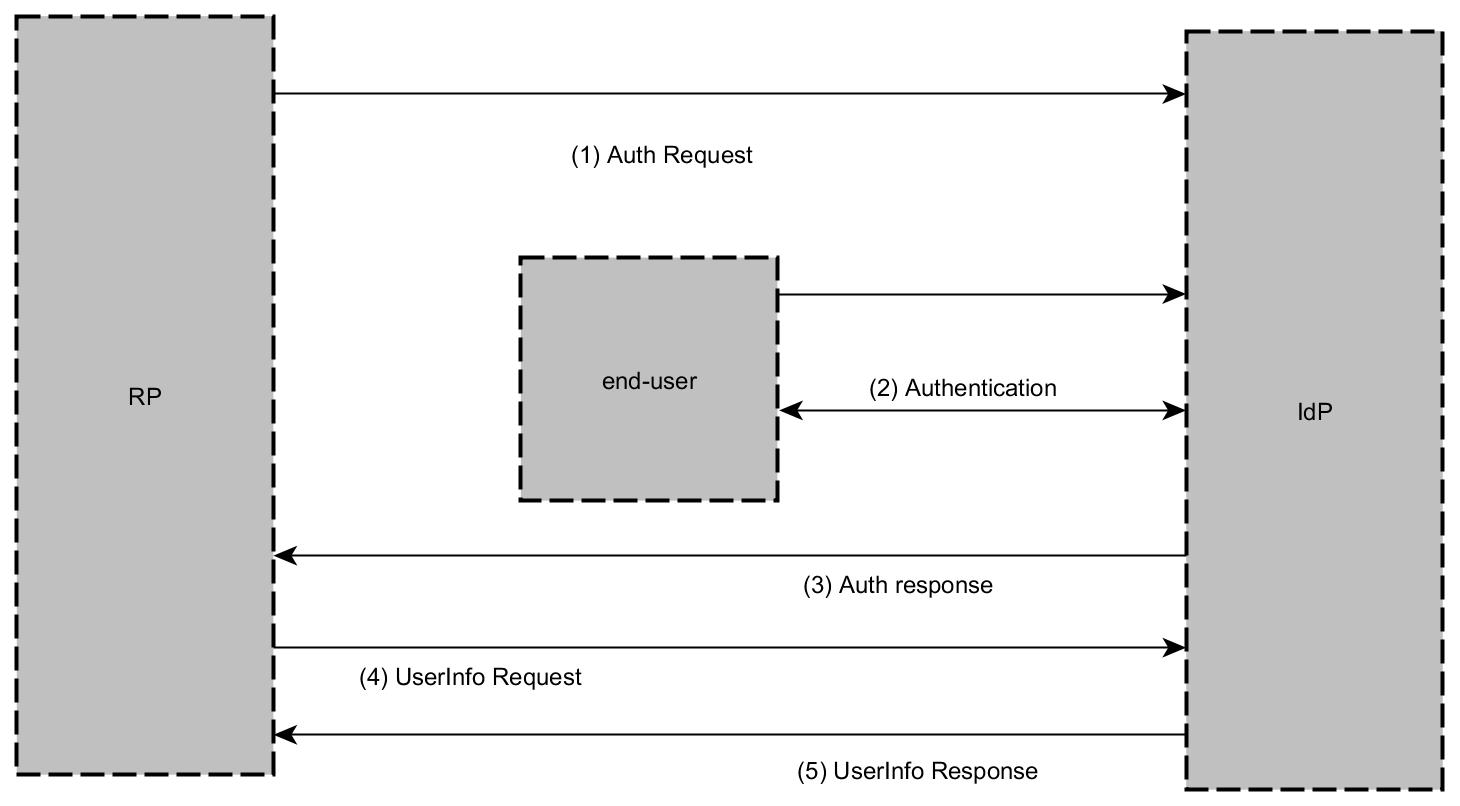
\includegraphics[scale=0.6]{images/openID_connect.jpg}
\end{figure}

The idea is the following: when a user wants to connect to a service RP, instead of creating an account, he can connect to a known and trusted Identity Provider OP (Google, Facebook, etc). 
\\(1)The RP can for that prepare an adequate authentication request and redirect the user to its identity provider with this authentication request (the user is first prompted to enter its OpenID, from which the RP identifies the OP, and then redirected). 
\\It must be here understood that the user is used as a way of conveying a message. End-User redirections are in general to be preferred to direct communication (between RP and IdP) because both the OP and RP must interact with the End-User (see step 2), which is made easier when the requests come from the End-User.
\\(2) The user authenticates to its OP and allows the OP to deliver some details about him (email, etc).
\\(3) An ID Token and (most of the time) Access Token are returned to the RP. Again, redirection of the user can be used. The ID Token is a security token that contains Claims about the authentication of the End-user. Typically, if the user is authenticated, when the authentication expires, etc. Once the RP gets this token, it can already open a session for the end-user.
\\(4) Ultimately, the RP can also asks for other pieces of information about the user (mail, etc) that it didn't have in the ID Token. For that, it will use its Access Token (security token for user information).
\\(5) User information is returned.

%A authorization code that he gives to the RP. \\With this code (one time code), the RP can ask the OP for an ID Token and an Access Token. The ID Token is a security token that contains Claims about the authentication of the End-user. Typically, if the user is authenticated, when the authentication expires, etc. Once the RP gets this token, it can already open a session for the end-user.\\



It is clear that it is a decentralized system, where entities can authenticate principals just by cooperating between each other and without having to ask a centralized authentication authority. Henceforth, except if the Identity Provider (or at least its administrators) maintains a list of accepted RPs, anybody can request the authentication of a user.
\\

OpenID 2.0 and Connect are nowadays broadly used, as in the new Google Login offer. But those 2 frameworks can be used in many ways and lead to numerous protocols.

The main difficulty behind such a system is indeed that OpenID is a framework, and not a protocol. The difference lies in the fact that an important part of the security measures are left to the one implementing the solution. Thus, it remains complicated to implement a reliable and secure protocol from this framework. It is possible though, to elaborate a robust system. 

Yu-Lin Jeng proposed for example an OpenID based framework for distributed authentication in a network where all nodes have the same pool of data and where users could access services from any node. His solution uses public OP and private OP, and is compliant to 3 three different types of authentication (among them LDAP)\cite{Jeng2012}.

E. Ghazizadeh et. al, have compared many openID based protocol and presented their own, resilient to Insider Attack, MITM, Phishing Attacks and DNS Poisoning at te same time, on the contrary to the other protocol \cite{Ghazizadeh}. Their solution included an OpenID layer on top of One Time Password OTP, Trusted Platform Module (TPM) hardware and the use of  SAML Token.

Some security flaws in OpenID Connect are also inherent to the OAuth 2.0 protocol and will be therefore detailed in the section \ref{02_OAuth}. 

\subsection{Other Approaches}
A lot of research has been done in the authentication field. This has led to numerous protocols, that we cannot detail here. However,  A. Liebl tried in 1994 to list the possible authentication protocols, his list is given in \hyperref[appendix:protocol_list]{appendix 1}. 

\section{Authorization}
\label{02_authorization}
According to the standard definition, authorization consists in granting to authenticated entities access rights to protected resources, with regards to a predefined access control policy.

Together with authentication and identification (who is exactly an authenticated user), authorization forms the constituting elements of Access Control, the selective restriction of access to a resource.

Often, the access controls models use the notion of \textit{owner} to control access to a resource, but other notions like roles, responsibilities or rules can be used.
 

\subsection{In a ditributed environement - OAuth 2.0}
\label{02_OAuth}

In a distributed environment, authorization might refer to some other notions. The most other common case is for example when an entity wants to be authorized to access a resource on behalf of another entity.

OAuth 2.0 is a recent framework, that corresponds to this need, and on which a lot of effort is put, and on which rely many famous security systems. It is for example the basis of the Facebook Login offer or the Google one. It is also the framework on which relies OpenID Connect (section \ref{02_OpenID}). It  is described as follows\cite{hardt2012oauth}: 

\begin{quote}
	The OAuth 2.0 authorization framework enables a third-party
	application to obtain limited access to an HTTP service, either on
	behalf of a resource owner by orchestrating an approval interaction
	between the resource owner and the HTTP service, or by allowing the
	third-party application to obtain access on its own behalf.
\end{quote}
Thus, still in \cite{hardt2012oauth}, 4 roles are defined:
\begin{itemize}
	\item \textbf{resource owner:} An entity capable of granting access to a protected resource.
	When the resource owner is a person, it is referred to as an
	end-user.
	\item \textbf{resource server:} The server hosting the protected resources, capable of accepting
	and responding to protected resource requests using access tokens.
	\item \textbf{client:} An application making protected resource requests on behalf of the
	resource owner and with its authorization.  The term "client" does
	not imply any particular implementation characteristics (e.g.,
	whether the application executes on a server, a desktop, or other
	devices).
	\item \textbf{authorization server:} The server issuing access tokens to the client after successfully
	authenticating the resource owner and obtaining authorization.
\end{itemize}

The principle of OAuth 2.0 is the following: the client first requests the Resource Owner approval to access the Resource (either directly, or indirectly through the authorization server). 
\\When it gets the Resource Owner authorization (under the form of an authorization grant), it can request to exchange this grant with an access token at the Authorization Server. 
\\Authentication is then performed by the server, and if the grant is valid, issues an access token, with which the user can access the Resource.
\\

As said above, the OAuth 2.0 protocol has been used and extended in many ways. OpenID Connect is based on it, as well as the previous versions of the Google Login and Facebook Login offers. However, several weaknesses have been found.

in 2012, S. Sun analyzed in detail the OAuth 2.0 framework, and exposed several of those weaknesses\cite{Sun2012}, like access token disclosure through network eavesdropping or cross-site scripting (XSS), impersonation of users, or Cross-site Request Forgery (CSRF). Most of the time, those weaknesses come from lacks in the security measures that implement the RPs. Indeed, like OpenID Connect, the framework is based on trust, which means among others that the IdPs must trust the RPs in regards to security implementation.

{\huge TODO: weaknesses}

\section{Security Framework Validation}
In order to verify that a framework responds to every security requirements, a certain methodology should be used. The following sections gives a few examples of such methodologies.

\subsection{BAN Logic}
